\part{Marchés et régulations} % (fold)
\label{prt:marches_et_regulations}

\section{Le marché et ses défaillances} % (fold)
\label{sec:le_marche_et_ses_defaillances}

Pourquoi la construction d'un marché européen était si importante ? Les lois de l'offre et la demande s'ajustent gracent à des variations du niveau des prix. Il est donc essentiel de préserver les marchés et la concurrence pour préserver les avantages des consomateurs. Cependant une ``bonne régulation'' est complexe, de part l'apparition de défaillances des marchés (entre autres) qui montrent que la marché concurrentiel n'est pas forcément la solution optimale. Par exemple selon Schumpetter les secteurs disposant de monopoles sont les plus à mènes d'innover.

\subsection{Concurrence parfaite} % (fold)
\label{sub:concurrence_parfaite}

Pareto montre qu'en concurrence pure et parfaite, l'équilibre se trouve à l'optimum de Pareto. Il se définit comme l'état dans lequel on ne peut améliorer le bien être d'un agent sans déteriorer celui d'au moins un autre. Cependant il faut que l'on soit en concurrence pure et parfaite qui implique : 

\begin{itemize}[label =\ding{69}]
	\item \textbf{Atomicité des participants :} L'action des participants n'a pas d'influence sur les quantités ni les prix, on dit qu'ils sont ``price takers''.
	\item \textbf{Homogénéité des biens :} Les acheteurs sont indifférents à l'identité des vendeurs, seul le prix importe.
	\item \textbf{Libre entrée et libre sortie du marché :} Tout acteur peut entrer et sortir d'un marché sans obstacles.
	\item \textbf{Information parfaite :} Tous les acteurs disposent d'une information parfaite du marché.
\end{itemize}
\begin{tcolorbox}[title=Concurrence pure et parfaite]

\subparagraph{Profit} % (fold)
\label{subp:profit}

\[
	\pi(Q)= pQ-CT(Q)
\]
\emph{avec $pQ$ les recettes et $CT(Q)$ le coût de production.}
% subparagraph profit (end)

\subparagraph{Profit moyen} % (fold)
\label{subp:profit_moyen}
\[
	\bar{\pi}= \frac{\pi}{Q}= p - CM(Q)
\]
\emph{avec $CM(Q)$ le coût moyen d'une unité.}


% subparagraph profit_moyen (end)

La maximisation du profit revient donc simplement à résoudre $\frac{\dif \pi}{\dif Q}=0 \Leftrightarrow p=C_m$ avec $C_m$ le côut marginal, c'est-à-dire la dérivée du coût total.
\end{tcolorbox}
% paragraph definitions_en_concurrence_pure_et_parfaite (end)

% subsection concurrence_parfaite (end)

\subsection{Défaillances de marché} % (fold)
\label{sub:defaillances_de_marche}
Plusieurs éléments peuvent mener à des défaillances des marchés, 
par exemple la présence d'un \emph{monopole}.
\begin{tcolorbox}[title=Monopole]


\[
	\pi(Q)= p(Q)Q- CT(Q)
\]

On maximise le profit: 
\[
	\frac{\dif \pi(Q)}{\dif Q}=0 \Leftrightarrow p(Q)+ Q\frac{\dif p(Q)}{\dif Q}= C_m \Leftrightarrow R_m= C_m
\]
\emph{Avec $R_m=p(Q)+ Q\frac{\dif p(Q)}{\dif Q}$}

On peut noter $R_m= \left(\frac{1}{\epsilon}+1 \right)p(Q)$ avec $\epsilon \leq -1$ l'elasticité des prix et on trouve ainsi : 
\[
	p(Q)_{\text{monopole}}=\frac{C_m}{\left(\frac{1}{\epsilon}+1 \right)} > C_m=p_{\text{concurrence}}
\]
\end{tcolorbox}
% paragraph definitions_en_situation_de_monopole (end)


% subsection defaillances_de_marche (end)

% section le_marche_et_ses_defaillances (end)

\section{Pouvoir des acteurs et structures des marchés} % (fold)
\label{sec:pouvoir_des_acteurs_et_structures_des_marches}

Lorsque la quantité d'acteurs et \emph{faible} sur un marché ils ont une \emph{influence sur les prix} en fonction de leur \emph{offre} et peuvent la quantifier à partir de $p(Q)$.

\subsection{Structure des marchés} % (fold)
\label{sub:structure_des_marches}

En \emph{concurrence monopolistique} les produits mêmes semblables sont suffisament 
différenciés pour bénéficier d'une position de monopole local. 
Les concurrents possèdent un pouvoir de marché basé sur un segment du produit.
\begin{tcolorbox}[title=Concurrence monopolistique]

Soit $n$ le nombre d'entreprises sur le marché, $p^*$ le prix moyen sur le marché,
$p$ le prix practiqué par la firme $i$, $Q$ la quantité totale offerte sur le marché 
et $Q_i$ les ventes de la firme $i$.

\[
	Q_i= Q\left(\frac{1}{n}-\beta (p-p^*)\right)
\]
$\beta$ est un coefficient mesurant variation des ventes suite à une variation du prix par rapport au prix moyen.

Le programme des firmes sur le marché est donc :
\[
	\underset{\max \, \pi_i}{Q_i}= p(Q_i)Q_i-cQ_i
\]
La fonction de demande inverse $p(Q_i)$ valant : 
\[
	p(Q_i)= \frac{1}{\beta}\left(\frac{1}{n}-\frac{Q_i}{Q}\right)+p^*
\]

La condition de premier ordre donne : 
\[
	c= \frac{1}{\beta}\left(\frac{1}{n}-2\frac{Q_i}{Q}\right)+p^*
\]
Dans le cas particulier ou toutes les entreprises sont identiques avec la même fonction de demande inverse on a $nQ_i=Q$ et donc $p=p^*$. De plus en utilisant le formule précedente on obtiens:
\[
	p=\frac{1}{\beta n}+c >c 
\]
Le prix d'équilibre est donc supérieur au côut marginal, l'entreprise reçoit donc un profit positif, cependant la concurrence fait baisser le prix. On pourrait de plus envisager la présence de coûts fixes CF, $CM=\frac{CF}{Q_i}+c$. Le profit de chaque firme si elle sont identiques s'écrit donc :
\[
	\pi = \frac{Q}{n} \left( \frac{1}{\beta n}+c- \left( n\frac{CF}{Q}+c \right) \right)
\]
Si on veut analyser \emph{l'équilibre de long terme} 
il faut analyser la situation \emph{d'annulation du profit} 
dans laquelle plus aucune entreprise entre sur le marché.
Soit
\[
	n^* = \sqrt{\frac{Q}{\beta CF}} \qquad p=\sqrt{\frac{CF}{\beta Q}}+c
\]
\end{tcolorbox}
% paragraph concurrence_monopolistique (end)
% subsection structure_des_marches (end)

Dans le cas ou le nombre d'acteurs sur le marché est trop faible l'hypothèse d'atomicité n'est plus vérifiée. Un type de marché très étudié est le duopole. 

\paragraph{Concurrence oligopolistique} % (fold)
\label{par:concurrence_oligopolistique}
 Sur les marchés en oligopole les entreprises se font concurrence et elles savent que leur comportement a un impact sur la marché. On voit donc apparaitre des interactions stratégiques entre les entreprises.
% paragraph concurrence_oligopolistique (end)

\subsection{Duopoles} % (fold)
\label{sub:duopoles}

On peut considérer plusieurs duopoles, si la concurrence se fait sur la \emph{quantité} 
on parle de \emph{duopole de Cournot} s'il y a symétrie de l'information
et \emph{duopole de Stackelberg} s'il y a asymétrie de l'information, 
si elle se fait sur le \emph{prix} on parle de \emph{duopole de Bertrand}.

\begin{tcolorbox}[title=Duopole de Cournot]
	
	On a $C_i=c_iq_i$ et la quantité totale de biens est $Q=q_1+q_2$, la fonction de demande inverse est $p(Q)=A-Q$.
	Chaque entreprise choisit une quantité $q_i$ en sachant que son profit dépend de cetter denière et de la quantité produite par sa concurrente.
	\[
		\pi_i = p(Q)q_i-C_i(q_i)
	\]
	La condition de premier ordre donne pour 1 (symétriquement pour 2) :
	\[
		q_1 = \frac{A-c_1}{2}-\frac{q_2}{2}
	\]
	Si on résout le problème impliquant les 2 fonctions de demande on peut trouver un équilibre dans lequel en considérant la quantité produite par sa concurrente on maximise notre profit.
	\[
		q_1^* = \frac{A-2c_1+c_2}{3} \Rightarrow p^* = \frac{A+c_1+c_2}{3} \quad \pi_i= \frac{(A+c_1+c_2)^2}{9}
	\]
	
\end{tcolorbox}

\begin{tcolorbox}[title=Duopole de Bertrand]
	
	Dans cette situation la demande dépend du prix proposé par chaque entreprise. On a : 
	\begin{align*}
		D_1 &= D(p_1), \quad D_2=0  &p_1<p_2 \\
		D_1 &= 0, \quad D_2 = D(p_2)  &p_1>p_2 \\
		D_1 &= D(p_1)/2 = D_2 &p_1=p_2
	\end{align*}
	Soit $C(q_i)=cq_i$ avec c le coût marginal le profit de l'entreprise 1 (symétriquement pour 2):
	\begin{align*}
		&\pi_1=0  &p_1&>p_2 \\
		&\pi_1 = \frac{(p_2-c)D(p2)}{2} &p_1&=p_2 \\
		&\pi_1= (p_2-\epsilon-c)D(p2-\epsilon) \approx (p_2-c)D(p2)> \frac{(p_2-c)D(p2)}{2} &p_1&=p_2-\epsilon
	\end{align*}
	Chaque entreprise va finalement baisser le prix jusqu'à arriver à $p=c$.
	
\end{tcolorbox}

Il existe aussi le cas de \emph{duopole asymétrique}, dans lequel les décisions sont prises séquentiellemt de part le caractère dominant de l'une des entreprises.

\begin{tcolorbox}[title=Duopole de Stackelberg]
	
  \begin{itemize}[label=\ding{71}]
		\item Le leader choisit de mettre sur la marché un quantité $q_1$.
		\item Le follower choisit $q_2$ maximisant sont profit en prenan en compte $q_1$.
	\end{itemize}
	Pour résoudre le programme on raisonne par backward induction. On maximise d'abord le profit du follower:
	\[
		\underset{\max q_2}{\pi_2} = p(q_1+q_2)q_2-C_2(q_2) \Rightarrow q_2= R_2(q1)= \frac{A-c_2}{2}-\frac{q_1}{2}
	\]
	Le leader conaissant la stratégie du follower maximise son profit:
	\[
		\underset{\max q_1}{\pi_1} = p(q_1+R_2(q1))q_2-C_1(q_1) \Rightarrow q_1= \frac{A-2c_1*c_2}{2}
	\]
	Il faut noter que le leader prend en compte 
  le fait que $q_2= R_2(q1)= \frac{A-c_2}{2}-\frac{q_1}{2}$.
	
	De plus on note que l'équilibre de Stackelberg donne pour le 
  leader un meilleur profit qu'en situation d'équilibre de Cournot. 
  Il vaut donc mieux avoir un position dominante.
\end{tcolorbox}

On note finalement que s'il y a \emph{libre entrée} sur un marché 
les entreprises vont entrer jusqu'à ce que les prix atteignent les \emph{coûts marginaux}.
% subsection duopoles (end)

\subsection{Discrimination par les prix} % (fold)
\label{sub:discrimination_par_les_prix}
 Pour réaliser une différenciation par les prix, il faut posséder un \emph{pouvoir de marché},
 les consomateurs doivent avoir des \emph{dispositions à payer différentes} 
 et les firmes doivent pouvoir les \emph{identifier}. 
 On distingue 3 types de discriminations : 
 
 \paragraph{La discrimination du premier degré:} % (fold)
 \label{par:la_discrimination_du_premier_degre}
 Vendre au prix maximal que le consomateur que chaque consomateur est disposé 
 à payer afin de profiter de l'ensemble des surplus consmateurs (maximaux) 
 
 % paragraph la_discrimination_du_premier_degre (end)
 
 \paragraph{Discrimination du troisième degré:} % (fold)
 \label{par:discrimination_du_troisieme_degre}
 On sectionne les consomateurs et on vend à des prix différents pour chaque partie 
 en maximisant le prix pour chaque secteur. On peut aussi éssayer d'attirer de nouveaux 
 clients en baissant les prix (cartes jeunes..).
 % paragraph discrimination_du_troisieme_degre (end)
 
 \paragraph{Discrimination du seconde degré:} % (fold)
 \label{par:discrimination_du_seconde_degre}
 On fait varier les prix en fonction des quantités achetées (packs), 
 la tarification est alors non linéaire (prix unitaire variable).
 

% paragraph discrimination_du_seconde_degre (end)

On peut classer la nécessité d'information de chaque discrimination (ordre croissant):
\[
	1^{er} > 3^{ème} > 2^{ème}
\]

Un caractère important pour réaliser la différenciation est de connaitre \textbf{l'elasticité}. On l'analyse en détail ci-dessous:

\begin{tcolorbox}[title=Élasticités]
	\begin{itemize}[label=\ding{69}]
		\item \textbf{Élasticité-prix de la demande :} elle mesure la sensibilité de la demande Q(p) à une variation de p. 
		\[
			\epsilon = \frac{\dif Q}{\dif p}\frac{p}{Q}
		\]
		Son signe est négatif (si prix augmente la demande diminue)
		\begin{tabular}{|c|c|c|}
		\hline
		$\epsilon$<-1 & $\epsilon \in$(-1,0) & $\epsilon =0$ \\
		\hline 
		élastique & faiblement élastique & inélastique \\
		\hline
		\end{tabular}
	
	
	
		\item \textbf{Élasticité-prix croisée :} elle permet d'analyser comment la demande d'un bien i va réagir à la variation de prix d'un bien.
		\[
			\epsilon_{ij} = \frac{\dif Q_i}{\dif p_j}\frac{p_j}{Q_i}
		\]
		\item \textbf{Élasticité-revenu de la demande:} analyse la variation de demande en fonction de la variation de revenu du consomateur.
		\[
			\epsilon_R = \frac{\dif Q}{\dif R}\frac{R}{Q}
		\]
	\end{itemize}
\end{tcolorbox}

On introduit de plus la notion de surplus consommateur : 
\begin{tcolorbox}[title=Surplus consommateur]
	La fonction de demande en fonction du prix permet de donner une évaluation du bénéfice réalisé par le consomateur. On note ce bénéfice $W(p^*)$, aussi nommé surplus, elle est simplement égale $v(q)-p*q*$ avec v la fonction de satisfaction du consomateur vérifiant $v'^{-1}(p)=q(p) \Leftrightarrow v'(q)=p(q)$. D'où :
	\[
		W(p^*)= \int_0^{q^*}p(q)\dif q - p^*q^* = \int_0^{q^*}v'(q)\dif q - p^*q^*
	\]
Une interprétation graphique de cette valeur es présenté sur la figure 1. On observe que l'on peut calculer cette valeur de la manière suivante :
\[
	W=(p(0)-p^*)q^*/2
\]

\end{tcolorbox}

\begin{figure}[h]
\begin{center}
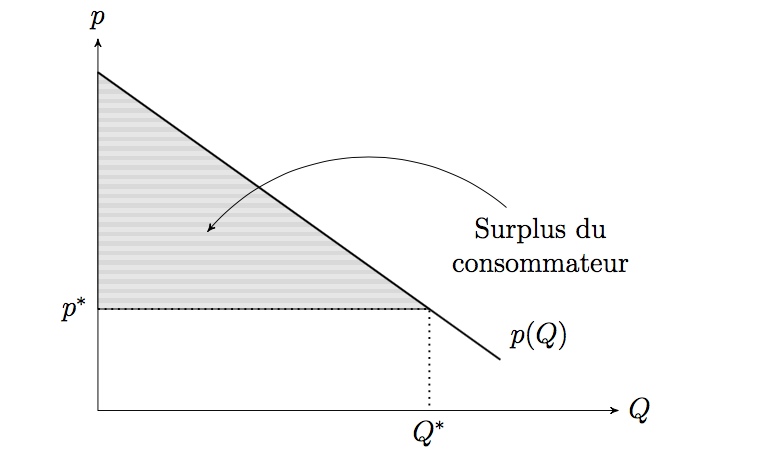
\includegraphics[scale=0.7]{./img/IM1}
\caption{Surplus du consomateur}
\end{center}
\end{figure}

% subsection discrimination_par_les_prix (end)

% section pouvoir_des_acteurs_et_structures_des_marches (end)

\section{Externalités positives et négatives} % (fold)
\label{sub:externalites_positives_et_negatives}

On parle d'externalités quand l'activité de consomation ou production d'un agent a une influence sur le bien être d'un autre sans faire l'effet d'une transaction économique. On présente 2 exemples :
\begin{itemize}
	\item Externalité positive : développement de nouvelles techniques scientifiques permet d'améliorer productivité ou aider dans la $R\&D$
	\item Externalité négative : pollution
\end{itemize}

Il faut pour définir les deux grands exemples d'externalités définir la rivalité et l'exclusion: 
\begin{itemize}
	\item Rivalité : un bien est rival s'il ne peut être utilisé par plusieurs agents en même temps.
	\item Exclusion : un bien est exclusif si on ne peut en disposer qu'en payant le prix.
\end{itemize}
Les biens publics (défense..) sont souvent non rivaux et non exclusifs au contraire des biens et services de consomation privée (mager une pomme..)

\subsection{L'innovation: une externalité positive} % (fold)
\label{sub:l_innovation_une_externalite_positive}

L'innovation a un caractère non rival et non exclusif mais présente plusieurs problèmes. Le premier si l'on investit dans l'innovation on est pas les seuls à en bénéficier. On ne peut s'approprier pleinement des résultats et de plus même si on acceptait cette contrainte on arriverait jamais à un taux suffisant pour bénéficier globalement à la société (non optimal). Le système des brevets est un solution partielle car elle bloque les innovations futures à partir de la notre (innovations nécessaires à d'autres innovations). 
% subsection l_innovation_une_externalite_positive (end)

\subsection{La pollution: une externalité négative} % (fold)
\label{sub:la_pollution_une_externalite_negative}

L'environnement étant "gratuit" les entreprises ne sont pas forcés de payer si elles l'endommagent ce qui répercute sur les riverains qui n'ont plus d'eau propre. Une solution les quotas de pollution cependant on crée un marché de revente de quotas. On peut émettre des taxes visant à élever le coût marginal des entreprise permettant d'obtenir une quantité optimale de produit et ainsi réduire la pollution (Pigou, 1920). Kyoto prévoyait un marché de quotas international, dans lequel à l'équilibre, les coûts marginaux de réduction de pollution sont égaux grâce aux différents prix des quotas d'un pays à l'autre (émissions réduites là ou c'est moins coûteux).

% subsection la_pollution_une_externalite_negative (end)
% section externalites_positives_et_negatives (end)
\section{Monopole naturel} % (fold)
\label{sec:monopole_naturel}

Une structure de monopole est clairement plus efficace lorsque les coûts fixes sont très élevés. Par exemple éléctricité... Il est plus éfficace de ne pas dupliquer le réseau dans ces cas la. L'état intervient souvent pour financer et controler l'entreprise qui fournit ce bien public, ce qui lui permet d'être propriétaire en tant qu'actionnaire unique et garant de l'intérêt général. L'Europe veut changer ce monopole institutionel en ouvrant la fourniture des services à des entreprises privées. Le modèle concurrentiel permet une amélioration constante des entreprises cependant on risque de voir une évasion des marchés moins rentables. Les entreprises déjà en place peuvent aussi éssayer de retarder l'entrée de la concurrence (ne pas réaliser d'investissements...)

% section monopole_naturel (end)

\section{Asymétries d'information} % (fold)
\label{sec:asymetries_d_information}

Dans les marchés réels il y a des asymétries d'information (un agent detient de l'info que l'autre n'a pas). Elles régissent les interactions entre agent. Soit un agent le principal qui demande à un agent mandataire de réaliser une tache, on peut trouver 2 types de phénomènes dûs à l'asymétrie d'information:
\begin{itemize}
	\item Sélection adverse : le principal ignore les caractéristiques du mandataire (par exemple fournisseur d'assurance ignore tout de son client).
	\item Aléa moral : le mandataire cache certains risques (par exemple déclarer des sinistrers non couverts ou changer sa façon de conduire une fois assuré)
\end{itemize}
% section asymetries_d_information (end)
\section{Concurrence et innovation} % (fold)
\label{sec:concurrence_et_innovation}

Schumpeter défend que le monopole est la structure de marché la plus approprié pour l'innovation car c'est la seule qui dégage assez de profits pour investir en recherche. Arrow dit qu'au contraire elle va s'accomoder ce sont les entreprises en compétition qui vont éssayer d'innover pour augmenter leurs profits. Gilbert cependant le contredit en disant que le monopole innove pour garder sa position de domination et ne pas inciter d'autres entreprises à entrer sur le marché. De récents travaux montrent que la concurrence est bonne pour l'innovation tant qu'elle ne force pas à trop diminuer les profits ce qui empècherait de financer la recherche.

% section concurrence_et_innovation (end)




% part marches_et_regulations (end)

